
\chapter{GCSE Revision: Functions and Function Transformation Questions}

\begin{enumerate}
  \item \mrk{3}
  \begin{figure}[H]
    \centering
    \textbf{A}
    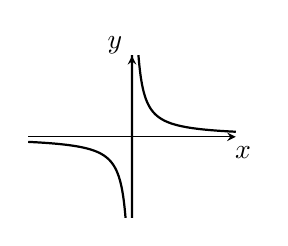
\begin{tikzpicture}
      \begin{axis}[
          xmin = -8, xmax = 8,
          ymin = -8, ymax = 8,
          xticklabels = {},
          yticklabels = {},
          xtick = {0},
          ytick = {0},
          axis lines = middle,
          height = 0.3\textwidth,
          x label style={at={(ticklabel* cs:0.95)},anchor=north west},
          y label style={at={(ticklabel* cs:0.95)},anchor=south east},
          xlabel = {$x$},
          ylabel = {$y$},
        ]
        % Plot a function
        \addplot[
          domain = -8:8,
          samples = 200,
          smooth,
          thick,
        ] {4/x};
      \end{axis}
    \end{tikzpicture}
    \hspace*{1cm}
    \textbf{B}
    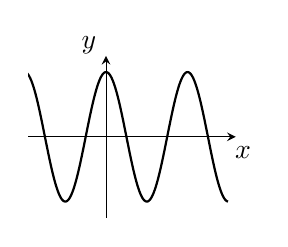
\begin{tikzpicture}
      \begin{axis}[
          xmin = -6, xmax = 10,
          ymin = -5, ymax = 5,
          xticklabels = {},
          yticklabels = {},
          xtick = {0},
          ytick = {0},
          axis lines = middle,
          height = 0.3\textwidth,
          x label style={at={(ticklabel* cs:0.95)},anchor=north west},
          y label style={at={(ticklabel* cs:0.95)},anchor=south east},
          xlabel = {$x$},
          ylabel = {$y$},
        ]
        % Plot a function
        \addplot[
          domain = -6.4:9.4,
          samples = 200,
          smooth,
          thick,
        ] {4*cos(deg(x))};
      \end{axis}
    \end{tikzpicture}\par
    \textbf{C}
    \begin{tikzpicture}
      \begin{axis}[
          xmin = -2, xmax = 1.5,
          ymin = -2, ymax = 6,
          xticklabels = {},
          yticklabels = {},
          xtick = {0},
          ytick = {0},
          axis lines = middle,
          height = 0.3\textwidth,
          x label style={at={(ticklabel* cs:0.95)},anchor=north west},
          y label style={at={(ticklabel* cs:0.95)},anchor=south east},
          xlabel = {$x$},
          ylabel = {$y$},
        ]
        % Plot a function
        \addplot[
          domain = -2:1,
          samples = 200,
          smooth,
          thick,
        ] {4*2^x};
      \end{axis}
    \end{tikzpicture}
    \hspace*{1cm}
    \textbf{D}
    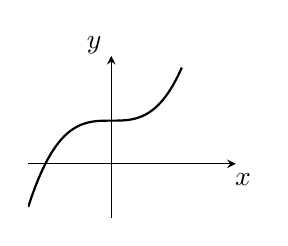
\begin{tikzpicture}
      \begin{axis}[
          xmin = -2, xmax = 3,
          ymin = -5, ymax = 10,
          xticklabels = {},
          yticklabels = {},
          xtick = {0},
          ytick = {0},
          axis lines = middle,
          height = 0.3\textwidth,
          x label style={at={(ticklabel* cs:0.95)},anchor=north west},
          y label style={at={(ticklabel* cs:0.95)},anchor=south east},
          xlabel = {$x$},
          ylabel = {$y$},
        ]
        % Plot a function
        \addplot[
          domain = -2:1.7,
          samples = 200,
          smooth,
          thick,
        ] {x^3+4};
      \end{axis}
    \end{tikzpicture}\par
    \textbf{E}
    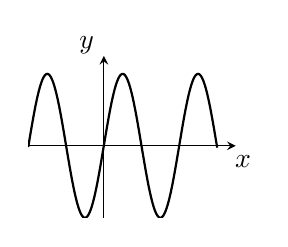
\begin{tikzpicture}
      \begin{axis}[
          xmin = -6.3, xmax = 11,
          ymin = -4, ymax = 5,
          xticklabels = {},
          yticklabels = {},
          xtick = {0},
          ytick = {0},
          axis lines = middle,
          height = 0.3\textwidth,
          x label style={at={(ticklabel* cs:0.95)},anchor=north west},
          y label style={at={(ticklabel* cs:0.95)},anchor=south east},
          xlabel = {$x$},
          ylabel = {$y$},
        ]
        % Plot a function
        \addplot[
          domain = -6.3:9.45,
          samples = 200,
          smooth,
          thick,
        ] {4*sin(deg(x))};
      \end{axis}
    \end{tikzpicture}
    \hspace*{1cm}
    \textbf{F}
    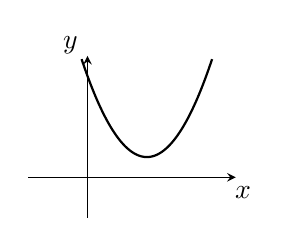
\begin{tikzpicture}
      \begin{axis}[
          xmin = -2, xmax = 5,
          ymin = -2, ymax = 6,
          xticklabels = {},
          yticklabels = {},
          xtick = {0},
          ytick = {0},
          axis lines = middle,
          height = 0.3\textwidth,
          x label style={at={(ticklabel* cs:0.95)},anchor=north west},
          y label style={at={(ticklabel* cs:0.95)},anchor=south east},
          xlabel = {$x$},
          ylabel = {$y$},
        ]
        % Plot a function
        \addplot[
          domain = -0.2:4.2,
          samples = 200,
          smooth,
          thick,
        ] {x^2-4*x+5};
      \end{axis}
    \end{tikzpicture}
  \end{figure}
  Each equation in the table represents one of the graphs \textbf{A} to \textbf{F}.\\
  Write the letter of each graph in the correct place in the table.

\end{enumerate}